\chapter{Numerical Results}

For simplicity of implementation, we demonstrate the results using pairs of steady-state models sharing the same states, mesh, and basis functions.

%------------------------------------------------------------------------------%
\section{Convection-Diffusion and Convection-Diffusion-Reaction Models}  %\label{sec:xx}
%------------------------------------------------------------------------------%

In this section, we demonstrate the method derived in Section \ref{sec:deriv} for two models in a 2D domain. In this case, the two models differ in the physics modeled. The high-fidelity model 
\begin{equation}
k_d\nabla^2 u - \vec{V}\cdot\nabla u + k_ru^2= f(q)
\end{equation}
is described by a single-species convection-diffusion-reaction equation with a nonlinear reaction term, where $k_d = 0.1$ is a diffusion coefficient and $k_r = -42.0$ is a reaction coefficient. The low-fidelity model
\begin{equation}
k_d\nabla^2 u - \vec{V}\cdot\nabla u + k_ru^2= f(q)
\end{equation}
differs only in the removal of reaction term. The velocity is described by $\vec{V}(x,y) = (2y(1-y),0)$, with the Peclet number everywhere in the domain $\Omega=[0,5]\times[0,1]$ small enough to make stabilization unnecessary. Homogeneous Dirichlet boundary conditions are used for simplicity. 

Given observations $d=(u(0.35,0.35),u(1.56,0.61),u(3.1,0.5))$ from three points in the domain, we wish to infer the forcing field $f(q)=q$ in order to calculate
\begin{equation}
I(q,u)=\int_{(x,y)\in \Omega_I} u \:\textrm{d}A,
\end{equation}
where $\Omega_I=[0.625,0.875]\times[0.375,0.625]$. The locations of the observations and the region $\Omega_I$ over which the QoI is calculated is shown in Figure \ref{fig:baseSetup}. Since the inverse problem is ill-posed, a Tikhonov regularization term $\frac{\beta}{2}\int_\Omega \|\nabla f(q)\|_2^2\:\textrm{d}A$ is used.

\begin{figure}[h]
\centering
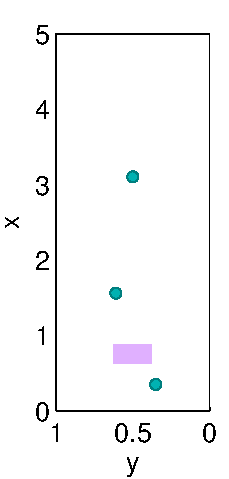
\includegraphics[width=0.8\textwidth]{baseSeries/setup_3_3.pdf}
\caption{Locations of observations and QoI region \red{ADD X TO AXIS...}}
\label{fig:baseSetup}
\end{figure}

Using the element-wise decomposition of (\ref{eq:finErrExp}), the proportion of the domain in which the high-fidelity model is used is increased until the estimated absolute relative error in the QoI is less than $1\%$. Figure \ref{fig:baseRef} shows the element-wise decomposition of the error estimate, as well as the areas of the domain where the low- and high-fidelity models were used. The true and estimated absolute relative errors in the QoI for these same intermediate models are shown in Figure \ref{fig:baseErr}, while the relative error in the error estimate is shown in Figure \ref{fig:baseErrErr}. %or effectivity index, since that's a standard for error estimates?
It can be seen that in this case, while the error estimates are not exact due to the nonlinear reaction term in the high-fidelity model, the error estimates are fairly accurate, and the QoI that would have been obtained from solving the inverse problem with the high-fidelity model can be replicated to within $1\%$ with a mixed-fidelity model where the high-fidelity model is used in only $20\%$ of the domain.

\begin{figure}[h]
\makebox[\textwidth]{%
    \begin{minipage}[t]{0.65\textwidth}
      \centering
      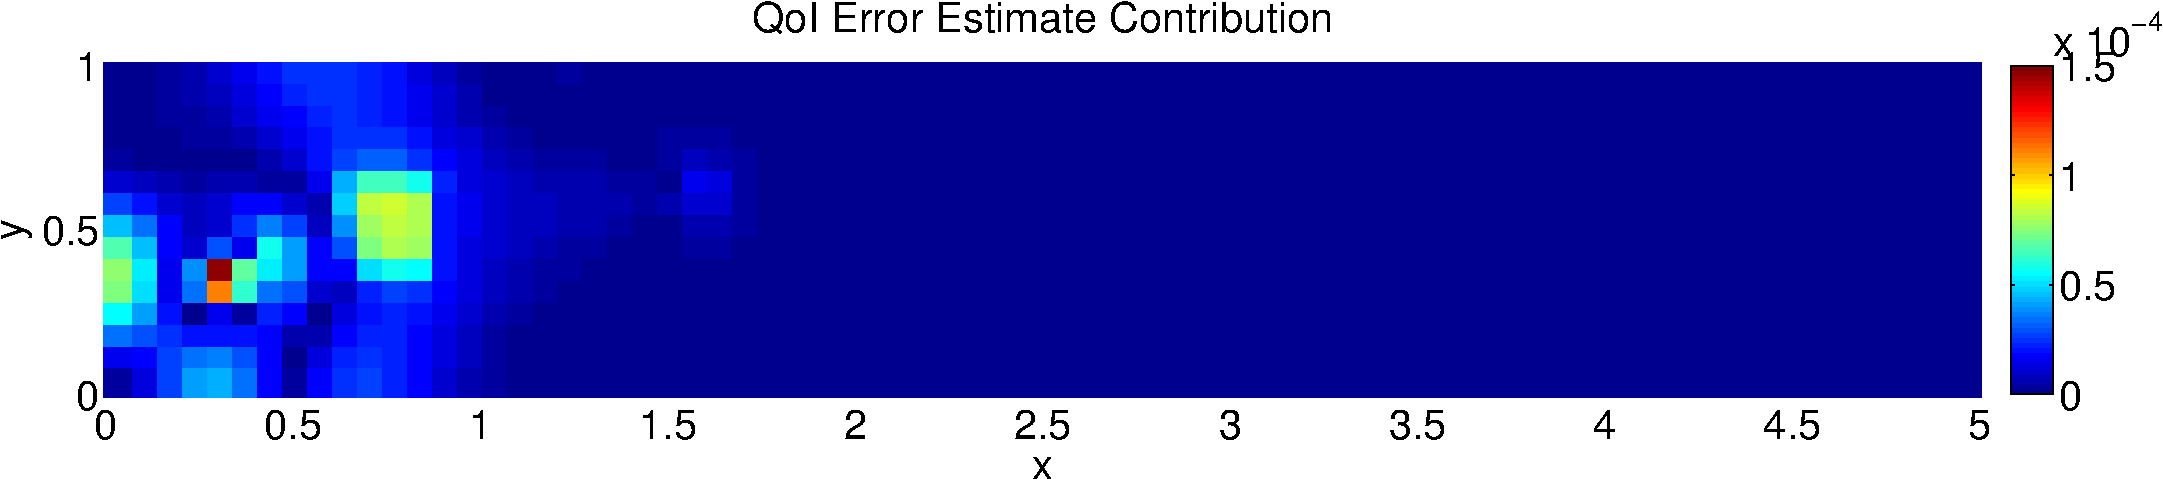
\includegraphics[width=\textwidth]{baseSeries/err_breakdown_LF.pdf}
    \end{minipage}%
    \hfill
    \begin{minipage}[t]{0.62\textwidth}
      \centering
      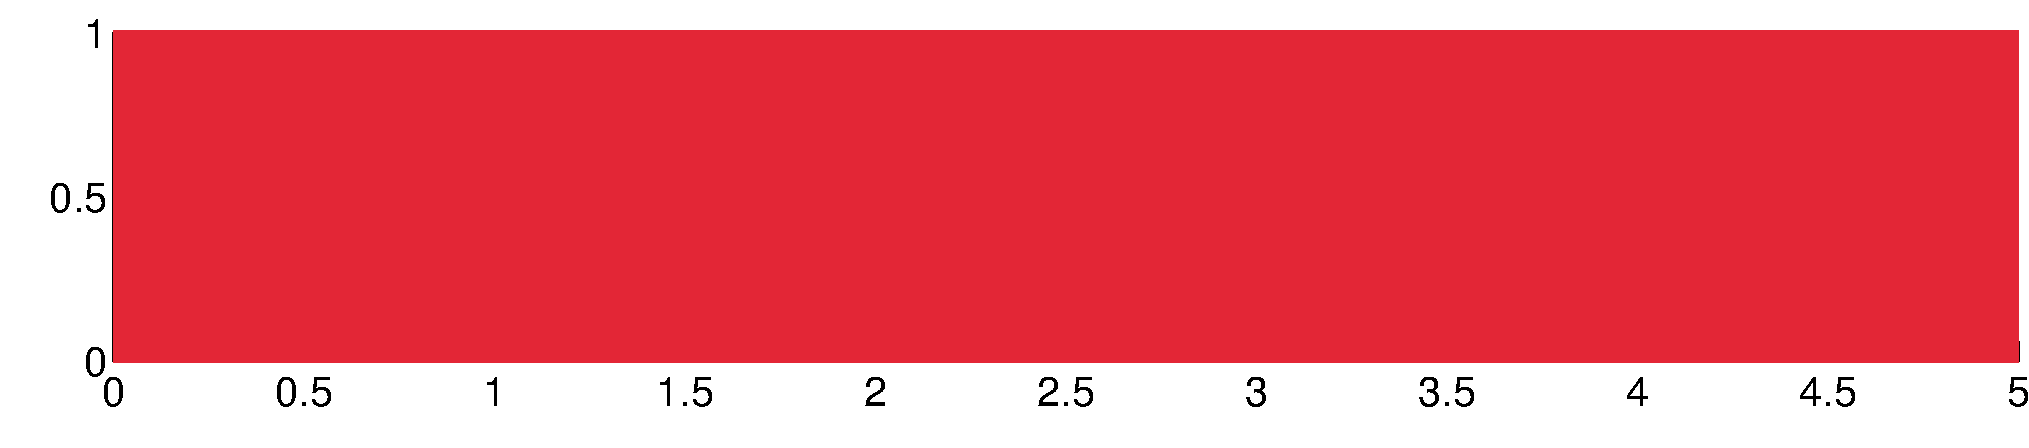
\includegraphics[width=\textwidth]{baseSeries/cd_cdr_LF_divvy.pdf}
    \end{minipage}%
    }
\makebox[\textwidth]{%
    \begin{minipage}[t]{0.65\textwidth}
      \centering
      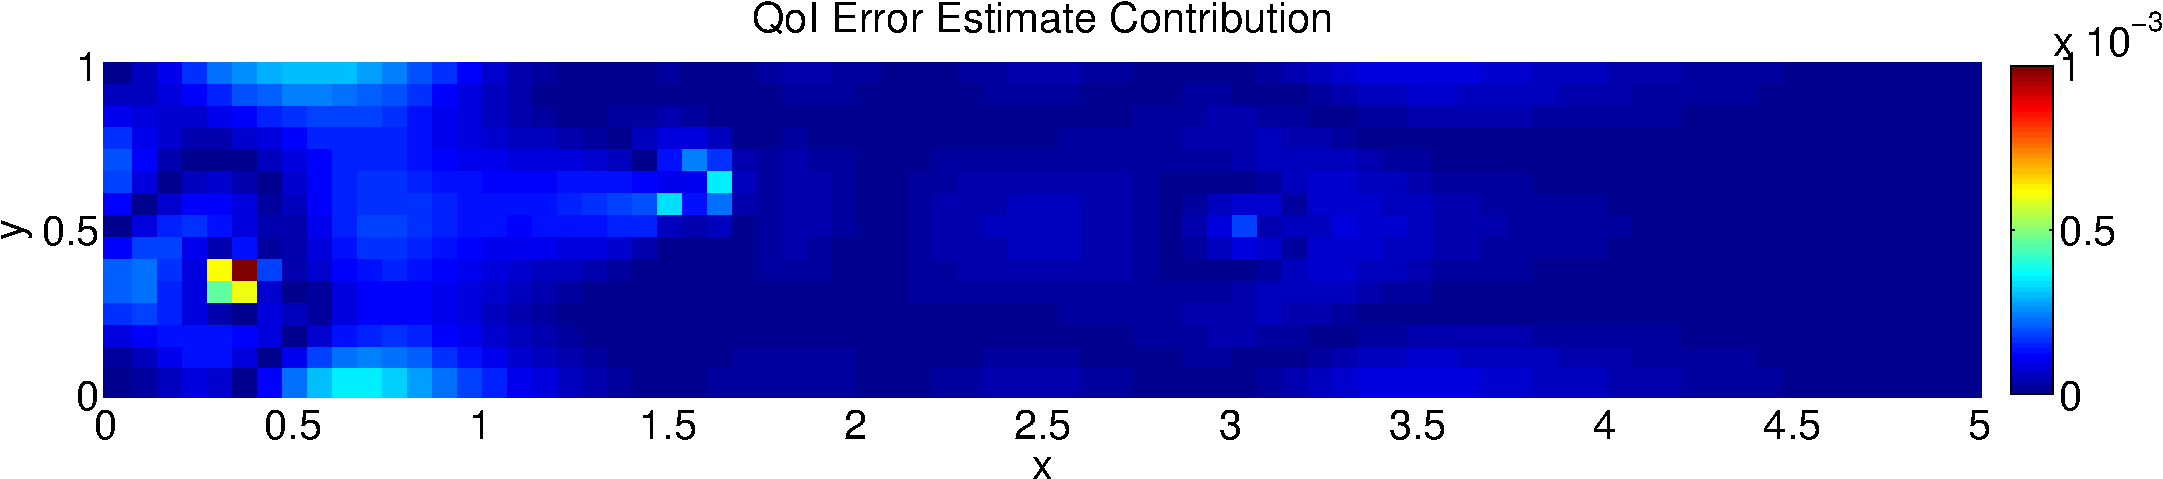
\includegraphics[width=\textwidth]{baseSeries/err_breakdown_MF01.pdf}
    \end{minipage}%
    \hfill
    \begin{minipage}[t]{0.62\textwidth}
      \centering
      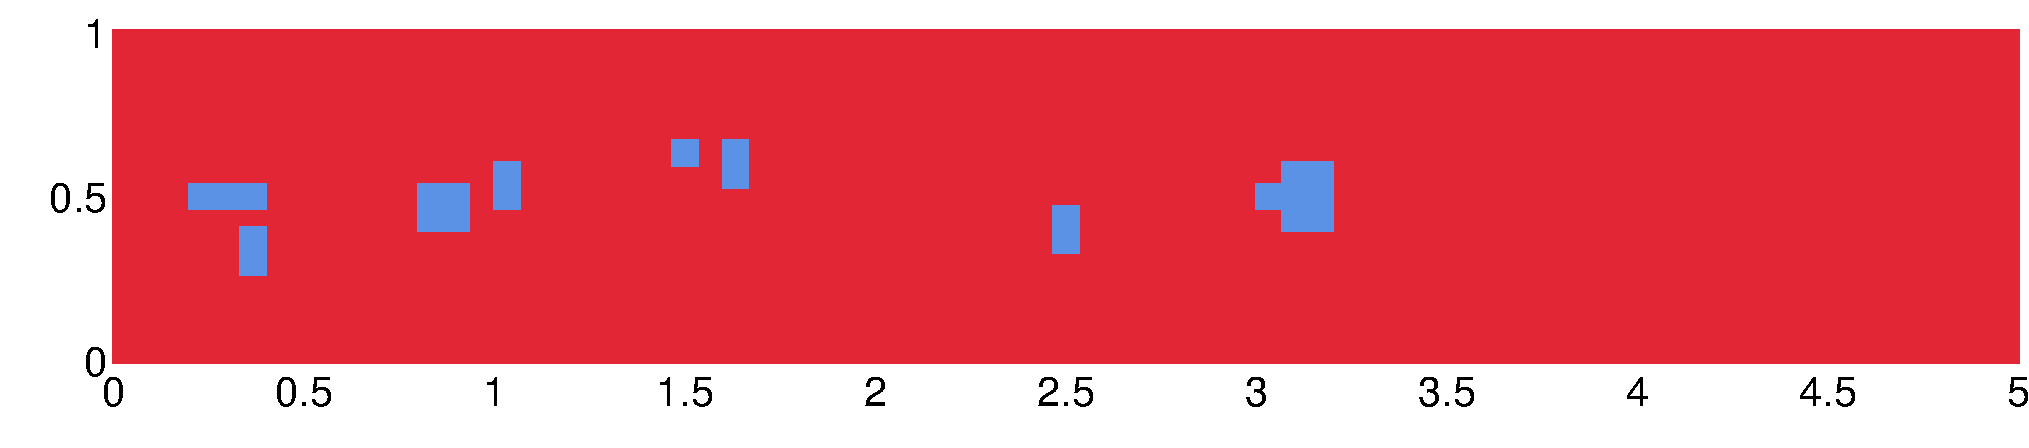
\includegraphics[width=\textwidth]{baseSeries/cd_cdr_MF01_divvy.pdf}
    \end{minipage}%
     }
\makebox[\textwidth]{%
    \begin{minipage}[t]{0.65\textwidth}
      \centering
      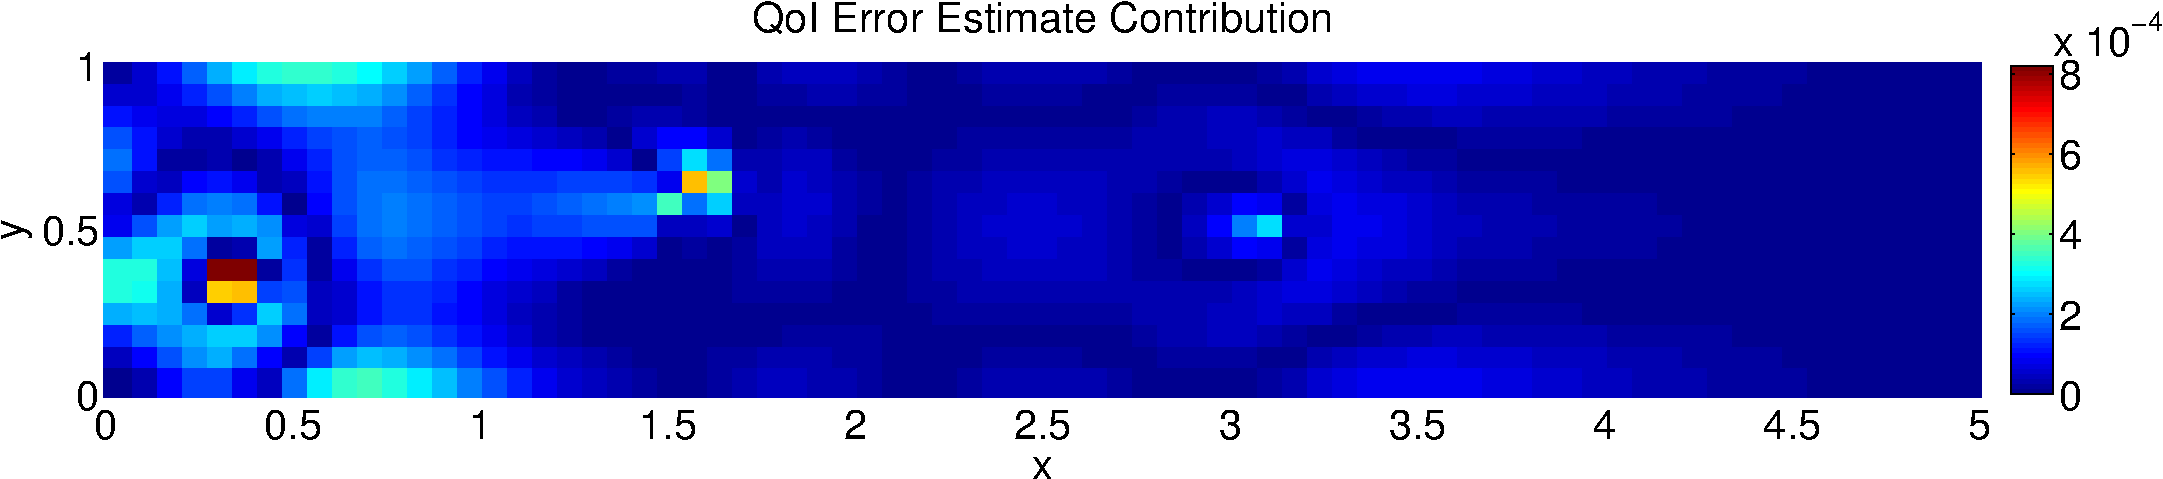
\includegraphics[width=\textwidth]{baseSeries/err_breakdown_MF02.pdf}
    \end{minipage}%
    \hfill
    \begin{minipage}[t]{0.62\textwidth}
      \centering
      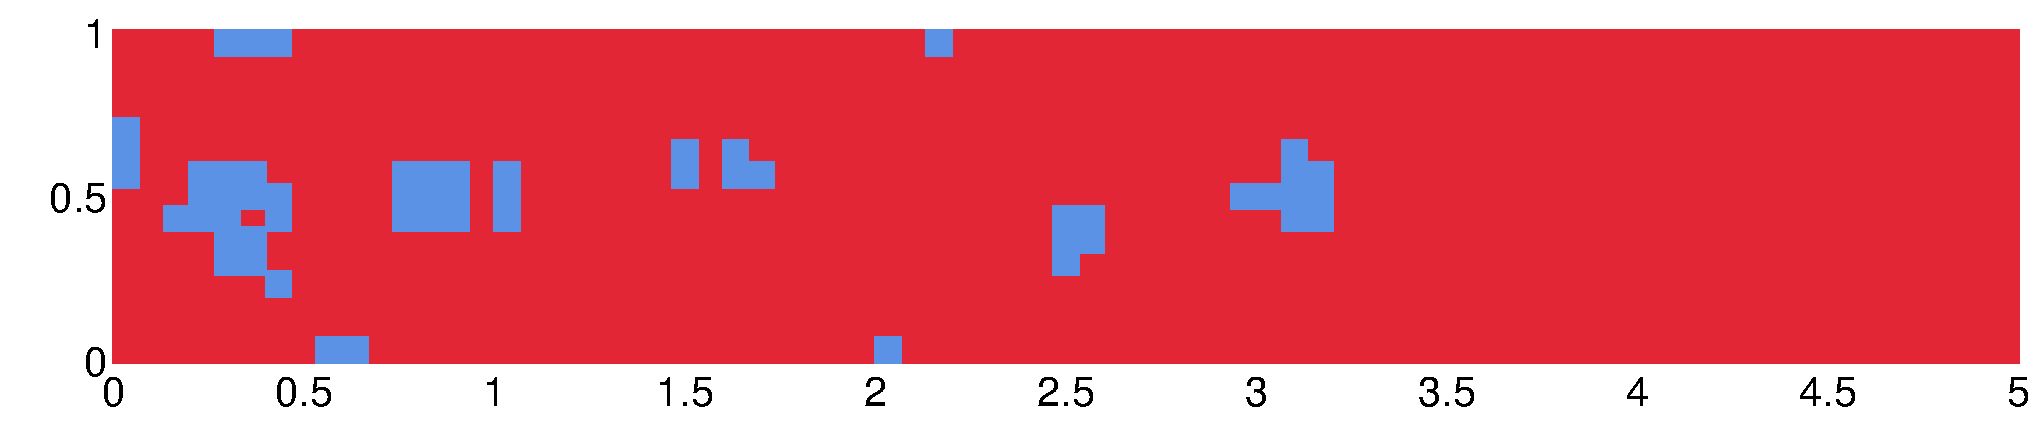
\includegraphics[width=\textwidth]{baseSeries/cd_cdr_MF02_divvy.pdf}
    \end{minipage}%
    }
\makebox[\textwidth]{%
    \begin{minipage}[t]{0.65\textwidth}
      \centering
      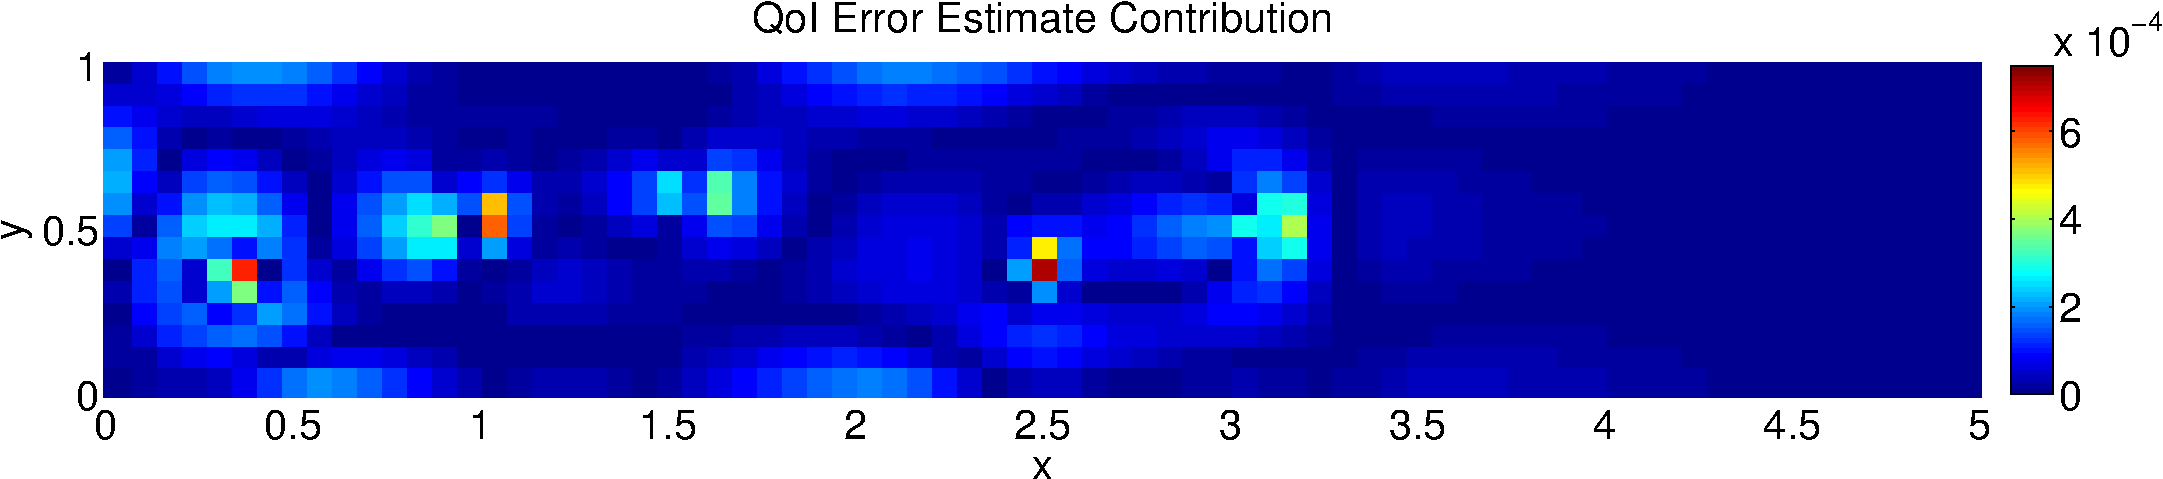
\includegraphics[width=\textwidth]{baseSeries/err_breakdown_MF03.pdf}
    \end{minipage}%
    \hfill
    \begin{minipage}[t]{0.62\textwidth}
      \centering
      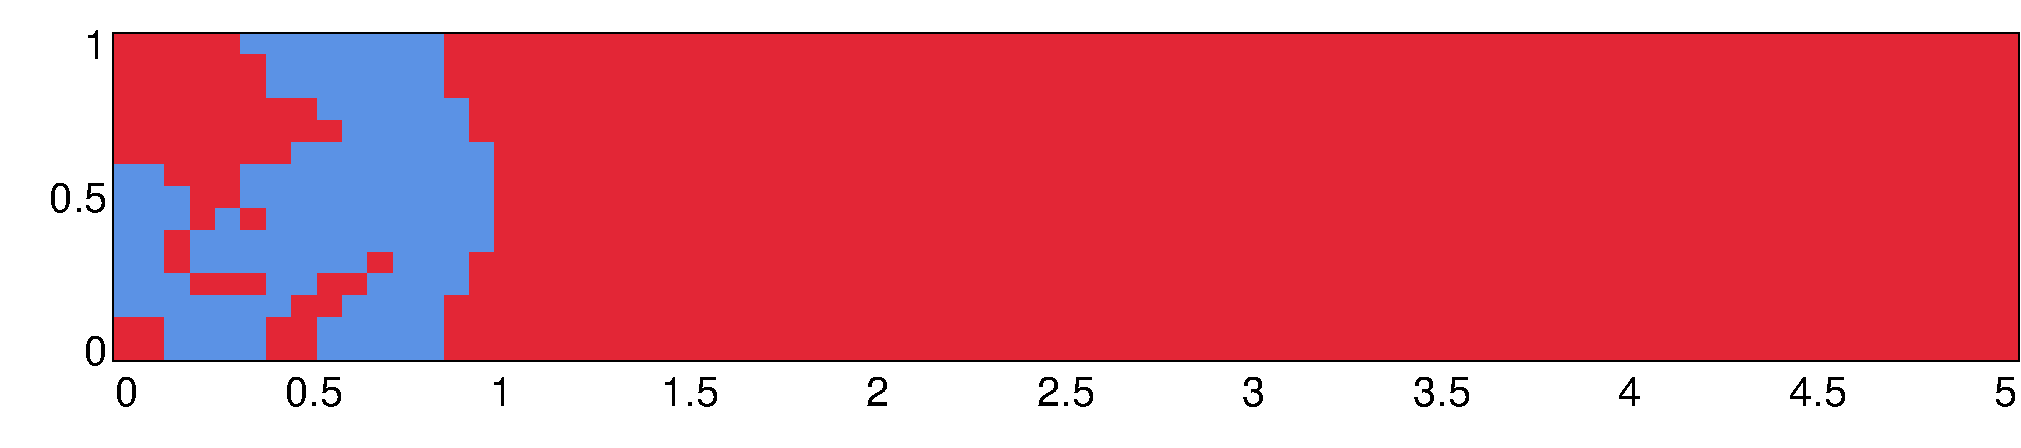
\includegraphics[width=\textwidth]{baseSeries/cd_cdr_MF03_divvy.pdf}
    \end{minipage}%
    }
\makebox[\textwidth]{%
    \begin{minipage}[t]{0.65\textwidth}
      \centering
      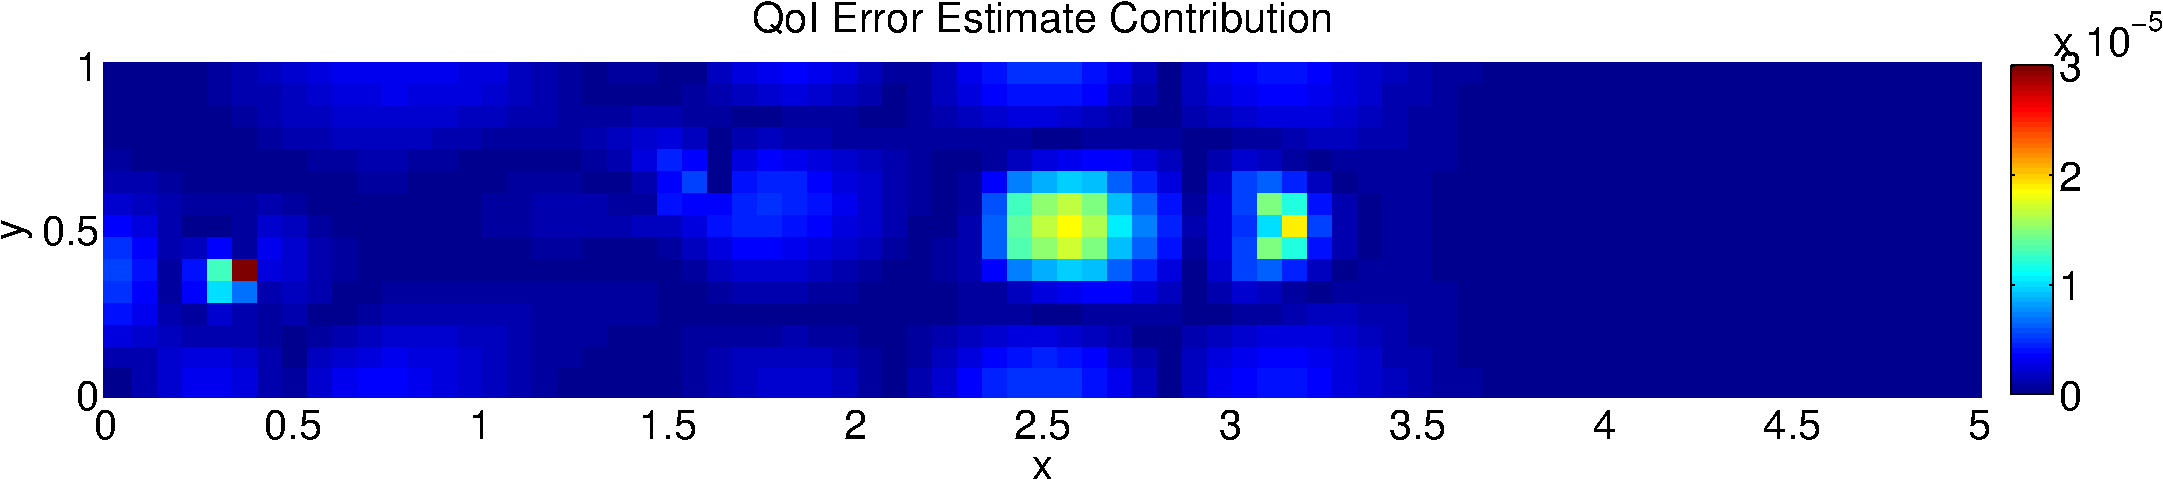
\includegraphics[width=\textwidth]{baseSeries/err_breakdown_MF04.pdf}
    \end{minipage}%
    \hfill
    \begin{minipage}[t]{0.62\textwidth}
      \centering
      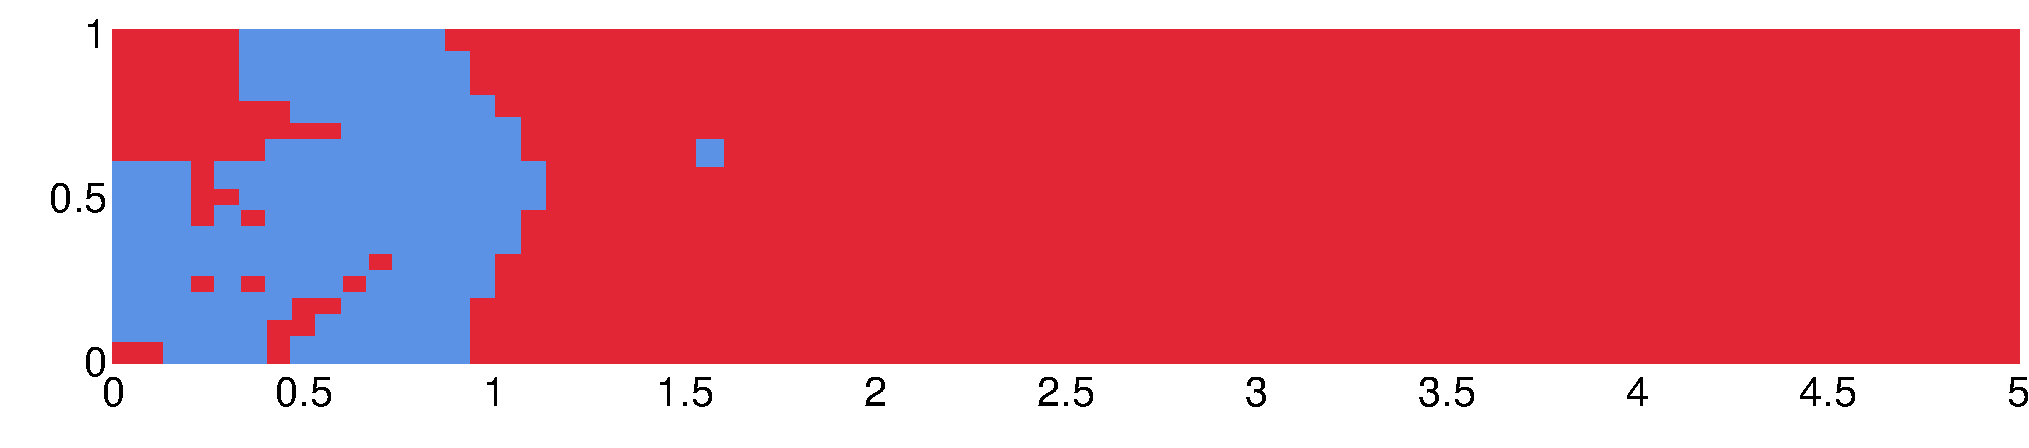
\includegraphics[width=\textwidth]{baseSeries/cd_cdr_MF04_divvy.pdf}
    \end{minipage}%
    }
\makebox[\textwidth]{%
    \begin{minipage}[t]{0.65\textwidth}
      \centering
      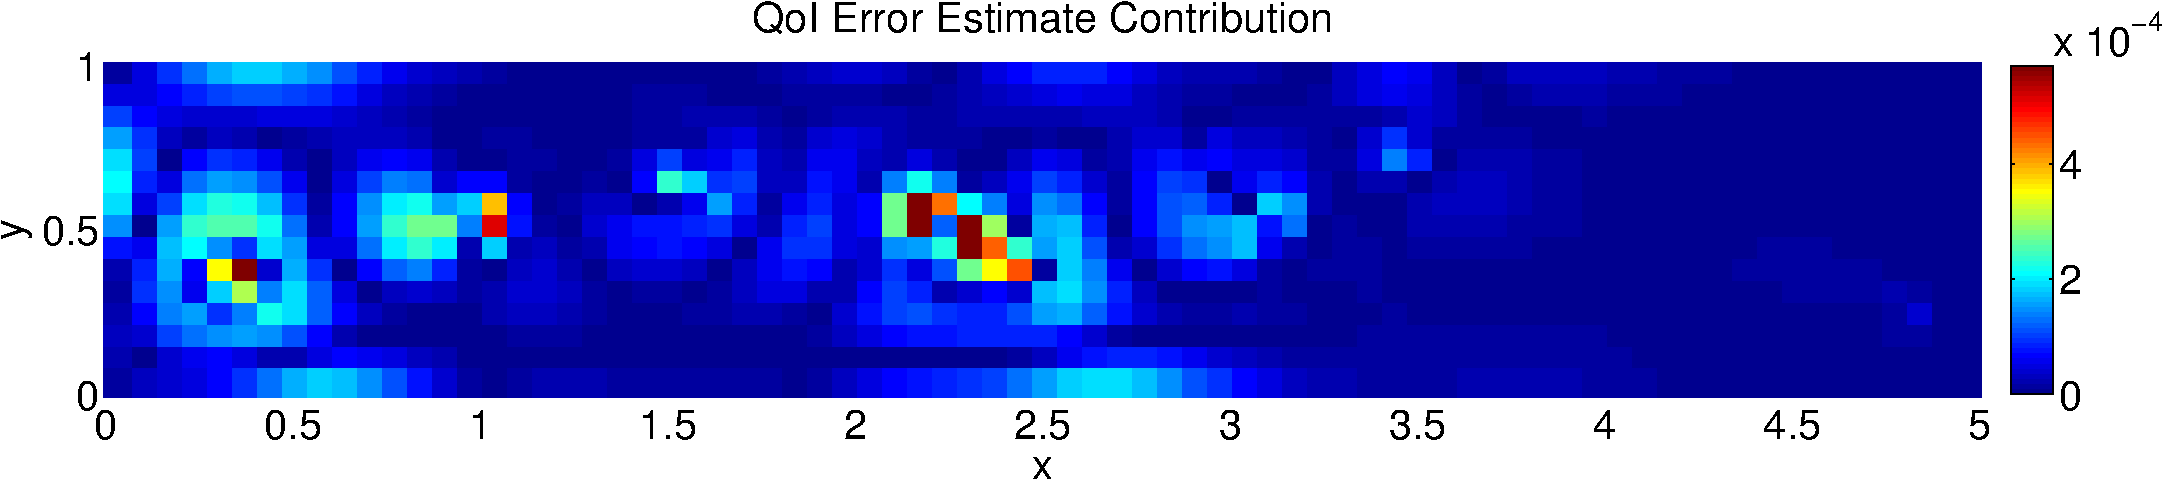
\includegraphics[width=\textwidth]{baseSeries/err_breakdown_MF05.pdf}
    \end{minipage}%
    \hfill
    \begin{minipage}[t]{0.62\textwidth}
      \centering
      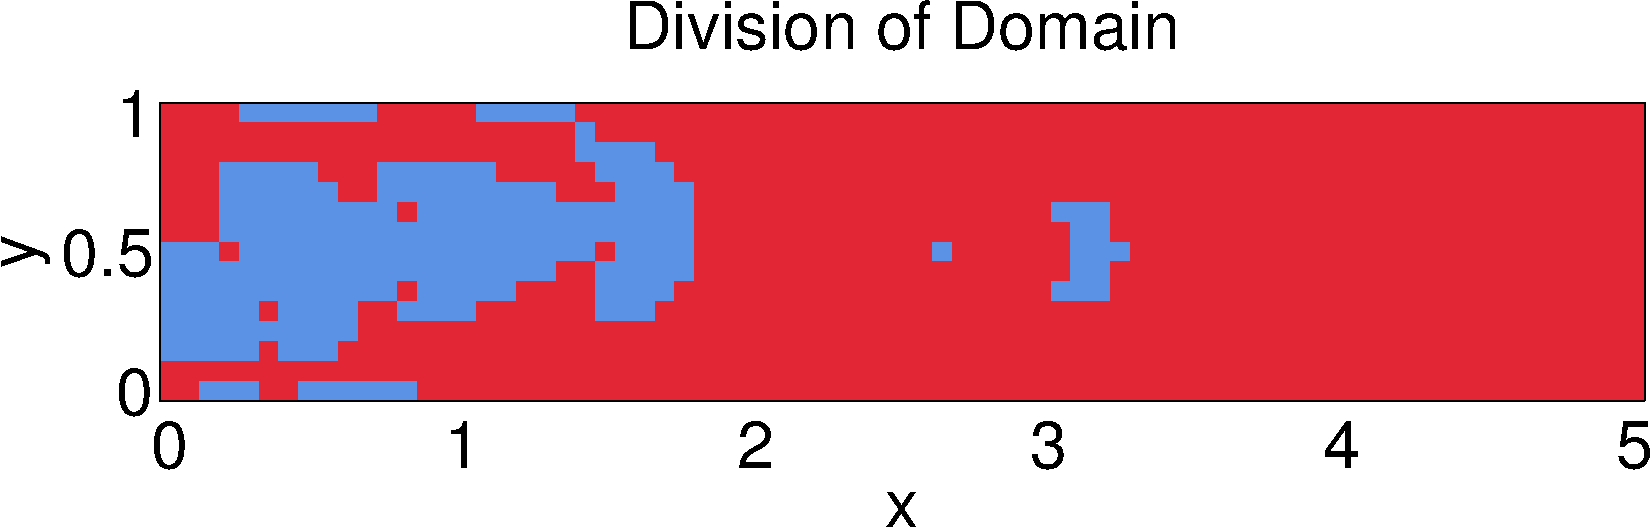
\includegraphics[width=\textwidth]{baseSeries/cd_cdr_MF05_divvy.pdf}
    \end{minipage}%
  }%
\caption{Model refinement series: element-wise breakdown of error estimates and corresponding subdomains (low-fidelity in red, high-fidelity in blue)}
\label{fig:baseRef}
\end{figure}

\begin{figure}[h]
\centering
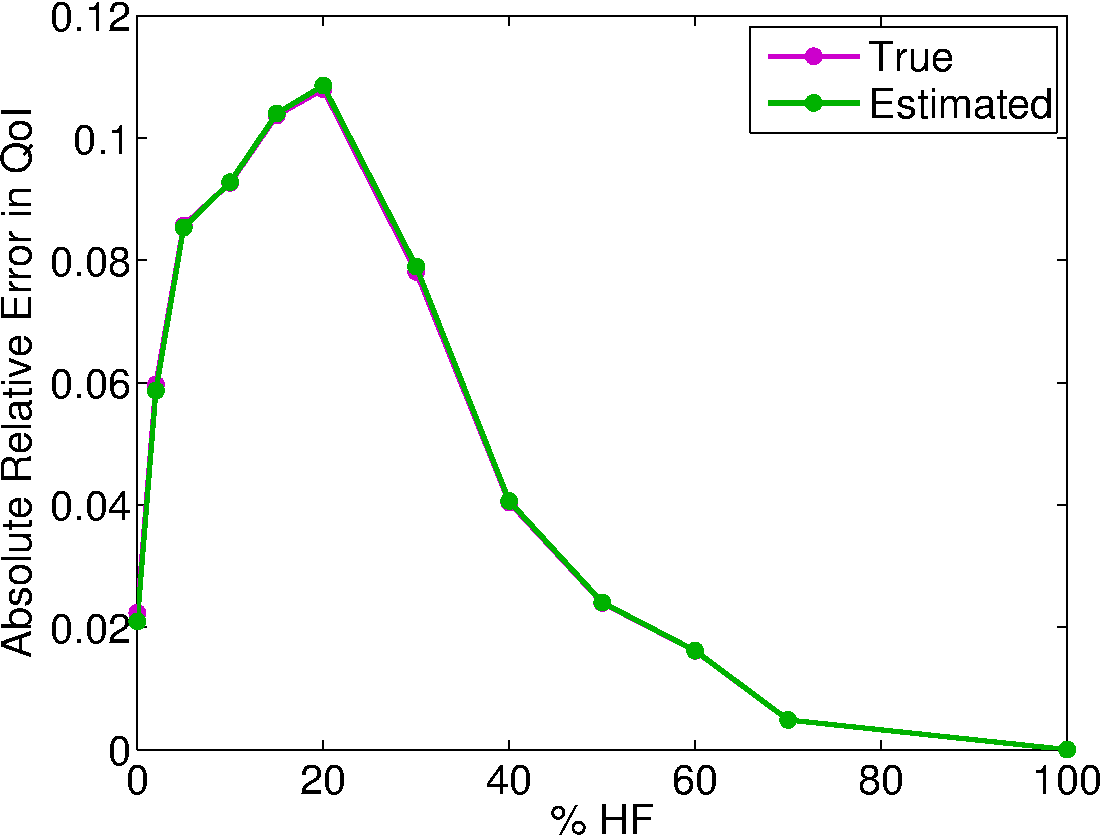
\includegraphics[width=0.8\textwidth]{baseSeries/err_est.pdf}
\caption{True and estimated absolute relative error in QoI}
\label{fig:baseErr}
\end{figure}

\begin{figure}[h]
\centering
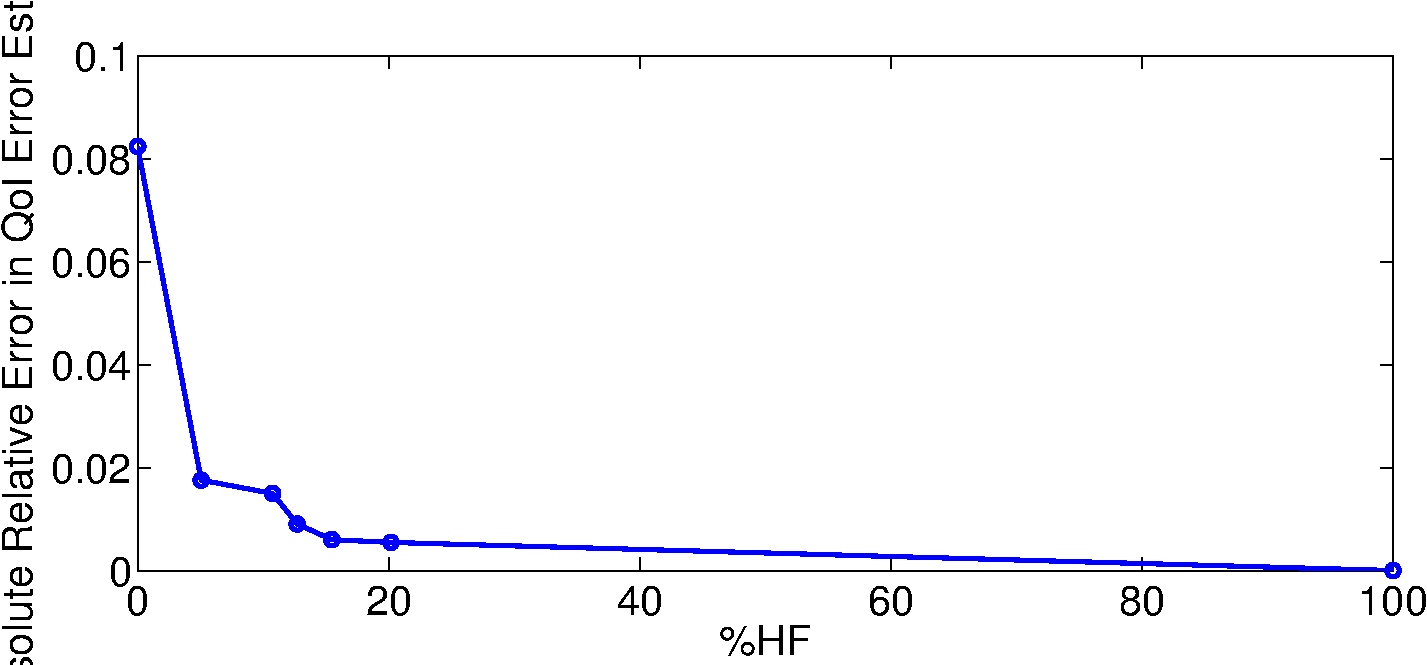
\includegraphics[width=0.8\textwidth]{baseSeries/err_err.pdf}
\caption{Absolute relative error in estimated absolute relative error in QoI \red{replace with table/graph of effectivity indices}}
\label{fig:baseErrErr}
\end{figure}

\subsection{Interaction of Observations and QoI}

The element-wise decomposition of the error estimate (\ref{eq:finErrExp}) suggests the use of the high-fidelity model in areas of the domain where \red{the parameter field?} is both informed by the observations and informative about the QoI. %can we only tie the physical domain and parameters so closely like this because these equations are localized (or what's the word...what hyperbolic equations don't have...something with "local"...)

To see this, we compare the element-wise decomposition of the error estimate for three sizes of the QoI region $\Omega_I$ given the same set of observations, and for three sets of observations given the same QoI region. Only the error estimate linearized about $\Psi_{LF}$ is shown in Figures \ref{fig:qoiStudy} and \ref{fig:dataStudy}; the later estimates have a similarly patterned decomposition.

\begin{figure}
\centering
\subfigure{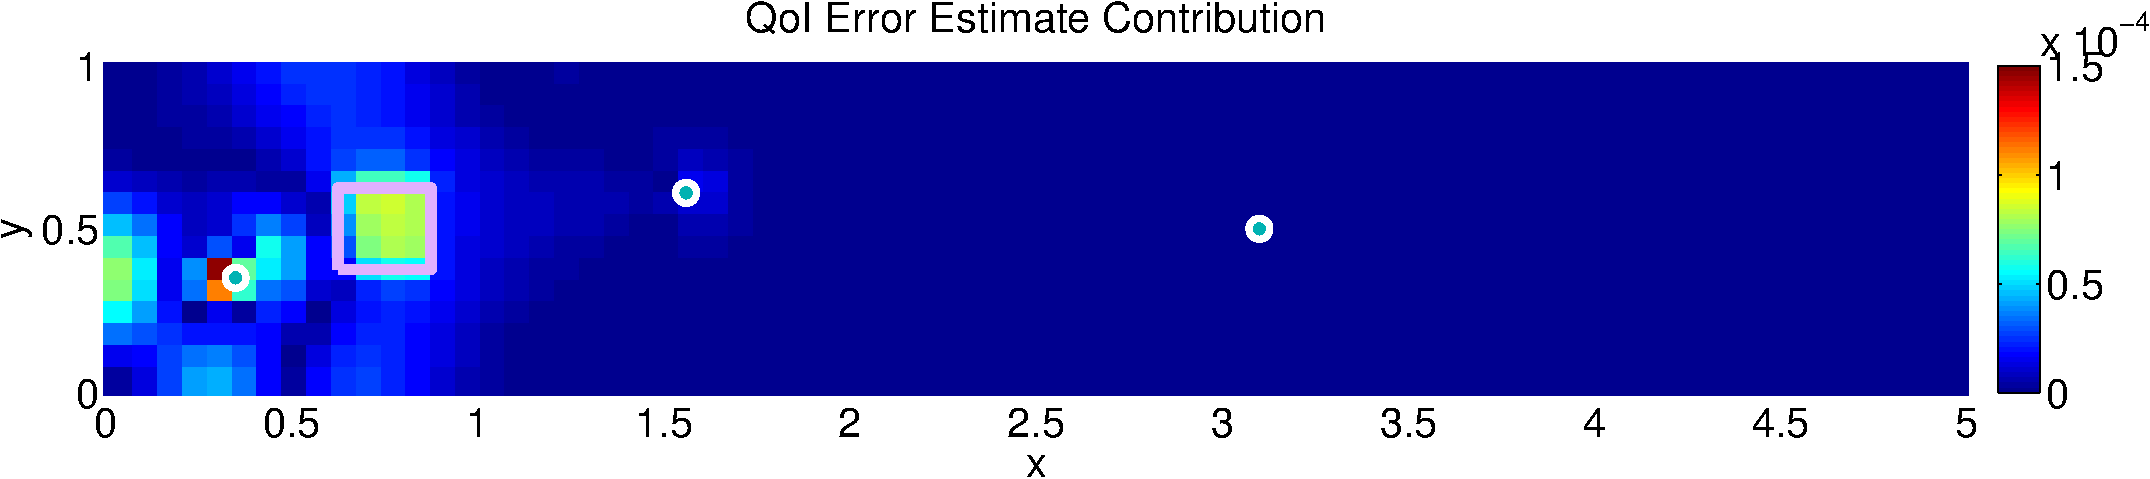
\includegraphics[width=0.8\textwidth]{vs_qoi/err_breakdown_3_3_study.pdf}}
\subfigure{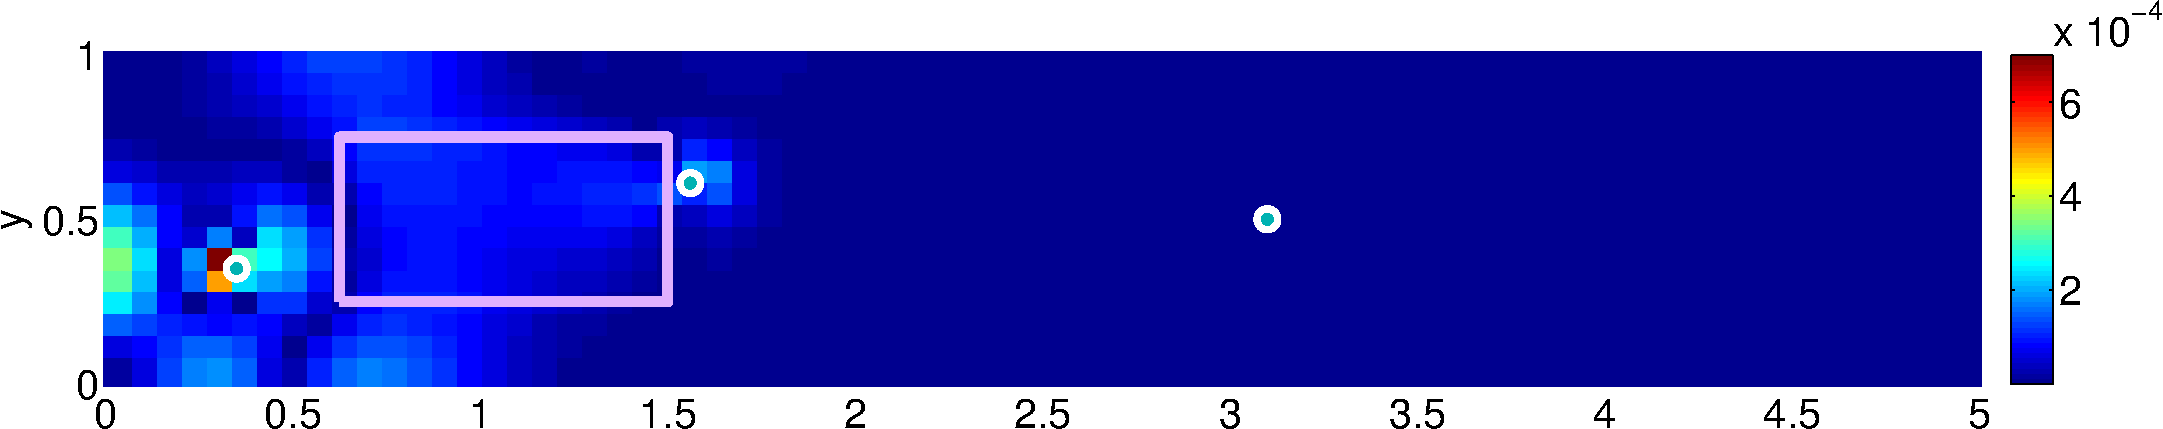
\includegraphics[width=0.8\textwidth]{vs_qoi/err_breakdown_7_3_study.pdf}}
\subfigure{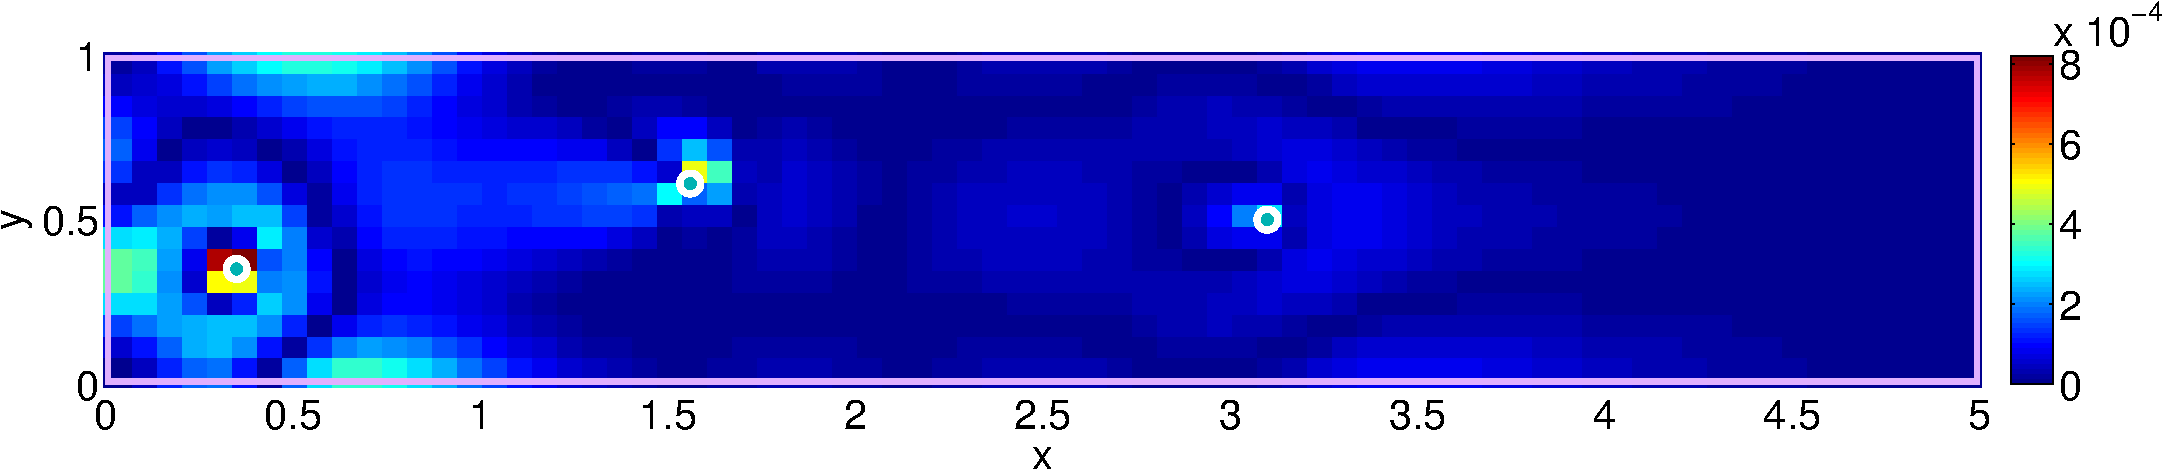
\includegraphics[width=0.8\textwidth]{vs_qoi/err_breakdown_5_3_study.pdf}}
\caption{Element-wise decomposition of error estimates for varying $\Omega_I$ (purple box) and same three observations (teal and white points)}
\label{fig:qoiStudy}
\end{figure}

\begin{figure}
\centering
\subfigure{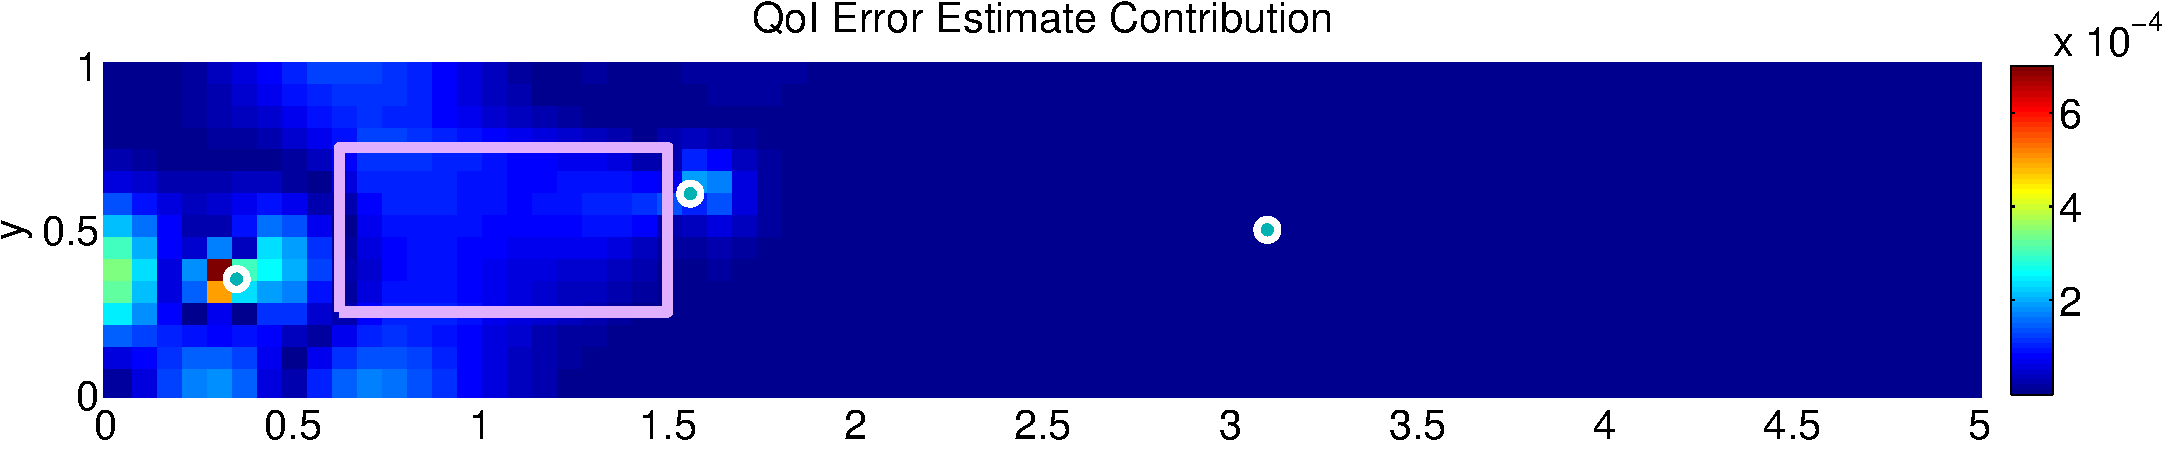
\includegraphics[width=0.8\textwidth]{vs_data/err_breakdown_7_3_studyv2.pdf}}
\subfigure{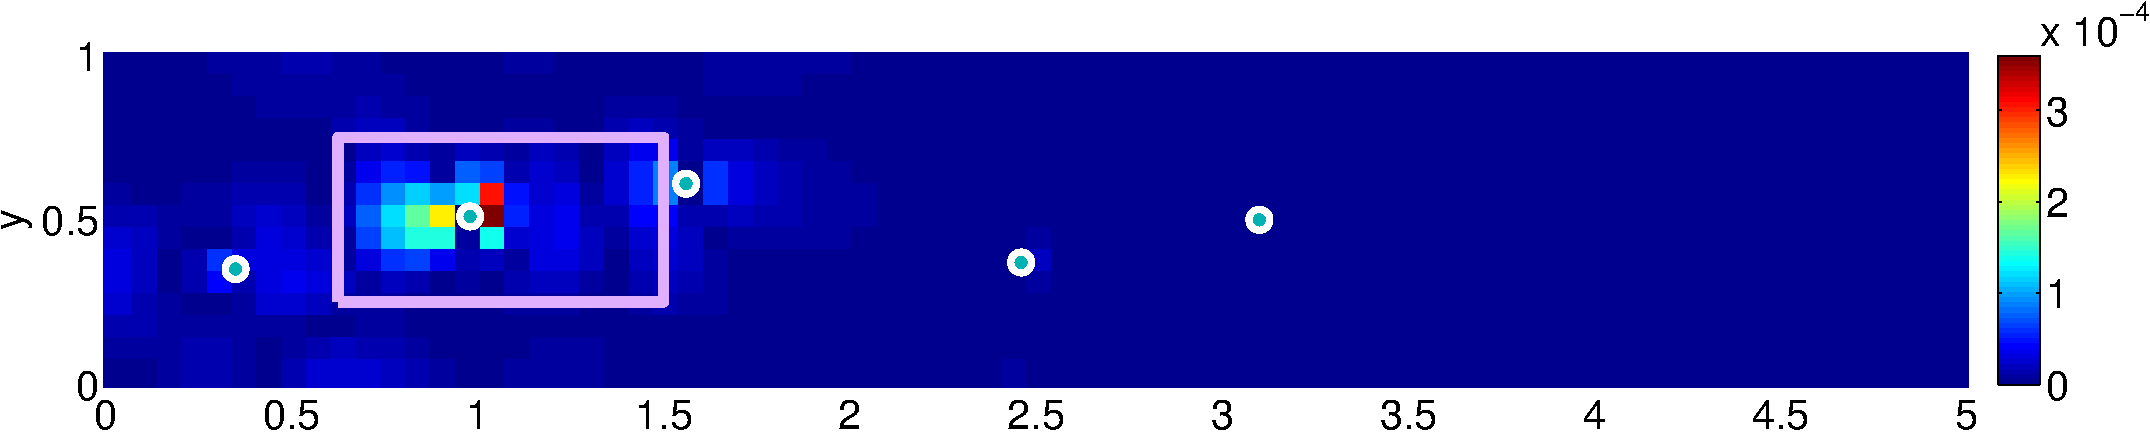
\includegraphics[width=0.8\textwidth]{vs_data/err_breakdown_7_5_study.pdf}}
\subfigure{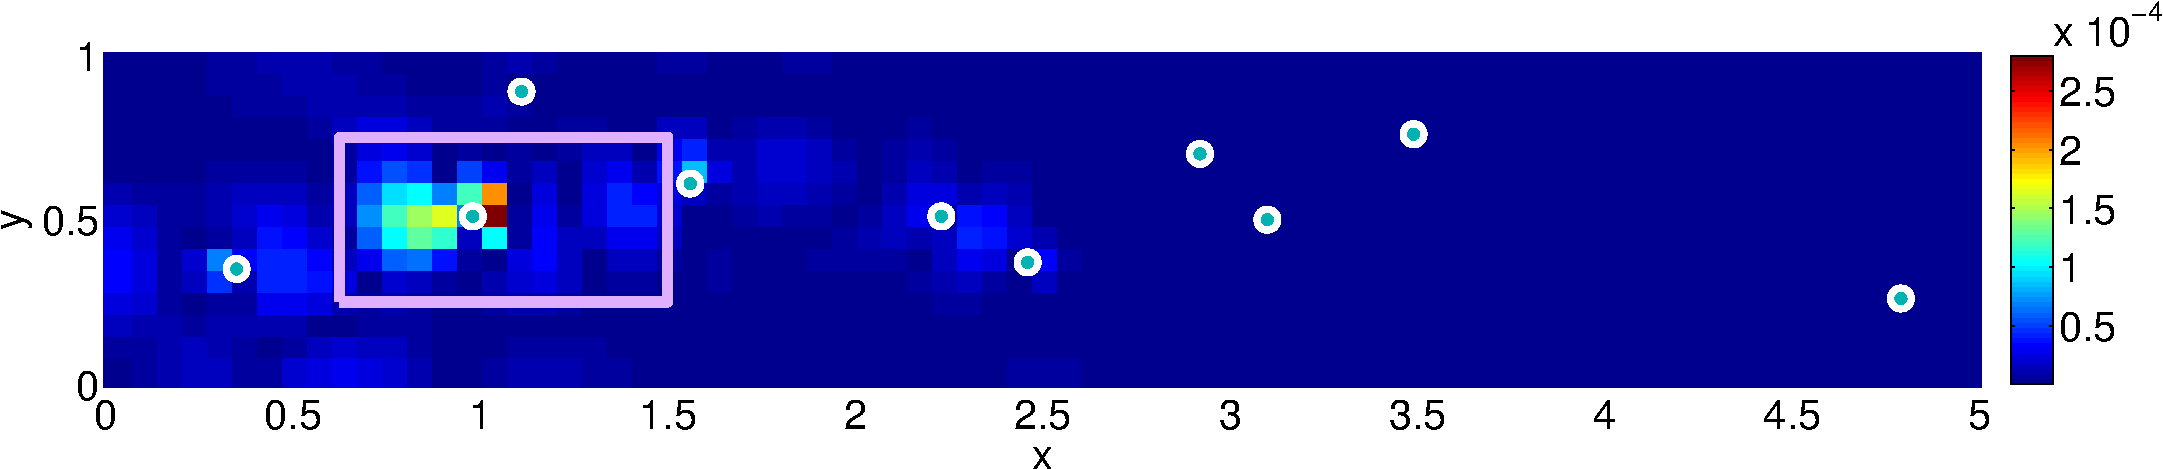
\includegraphics[width=0.8\textwidth]{vs_data/err_breakdown_7_10_study.pdf}}
\caption{Element-wise decomposition of error estimates for varying observations (teal and white points) and same $\Omega_I$ (purple box)}
\label{fig:datStudy}
\end{figure}

These results agree with intuition, and in this case an appropriate mixed-fidelity model could have been designed by intuition. In fact, this is a case in which the models are simple enough that it is actually cheaper to solve the inverse problem with the high-fidelity model than to rigorously form a mixed-fidelity model with which to solve the inverse problem instead. The interaction between the observations and the QoI need not always be obvious, however, as might be the case for \red{what?} models, and it is in these cases that a rigorous method for forming a mixed-fidelity model would be most helpful.

\subsection{Effect of Regularization}

As the magnitude of the regularization parameter $\beta$ it increased, the error estimate seems to indicate that whether the low- or high-fidelity model is used becomes less and less important in most of the domain, except in small areas around the most relevant observations. This behavior is expected\red{, or maybe I've just stared at this too often}. As $\beta$ increases, the regularization more strongly influences the parameter field that is inferred, although the regularization does not completely determine the inferred parameters and the observations still influence the inferred parameter field in the area around them; the choice of model in the QoI region becomes less important as the inferred parameter field in that area becomes more determined by regularization. 

The element-wise decomposition for the observations and QoI region shown in Figure \ref{fig:baseSetup} are shown in Figure \ref{fig:regStudy} for three values of the regularization parameter $\beta$. Only the error estimate linearized about $\Psi_{LF}$ is shown; the later estimates have a similarly patterned decomposition.

\begin{figure}
\centering
\subfigure{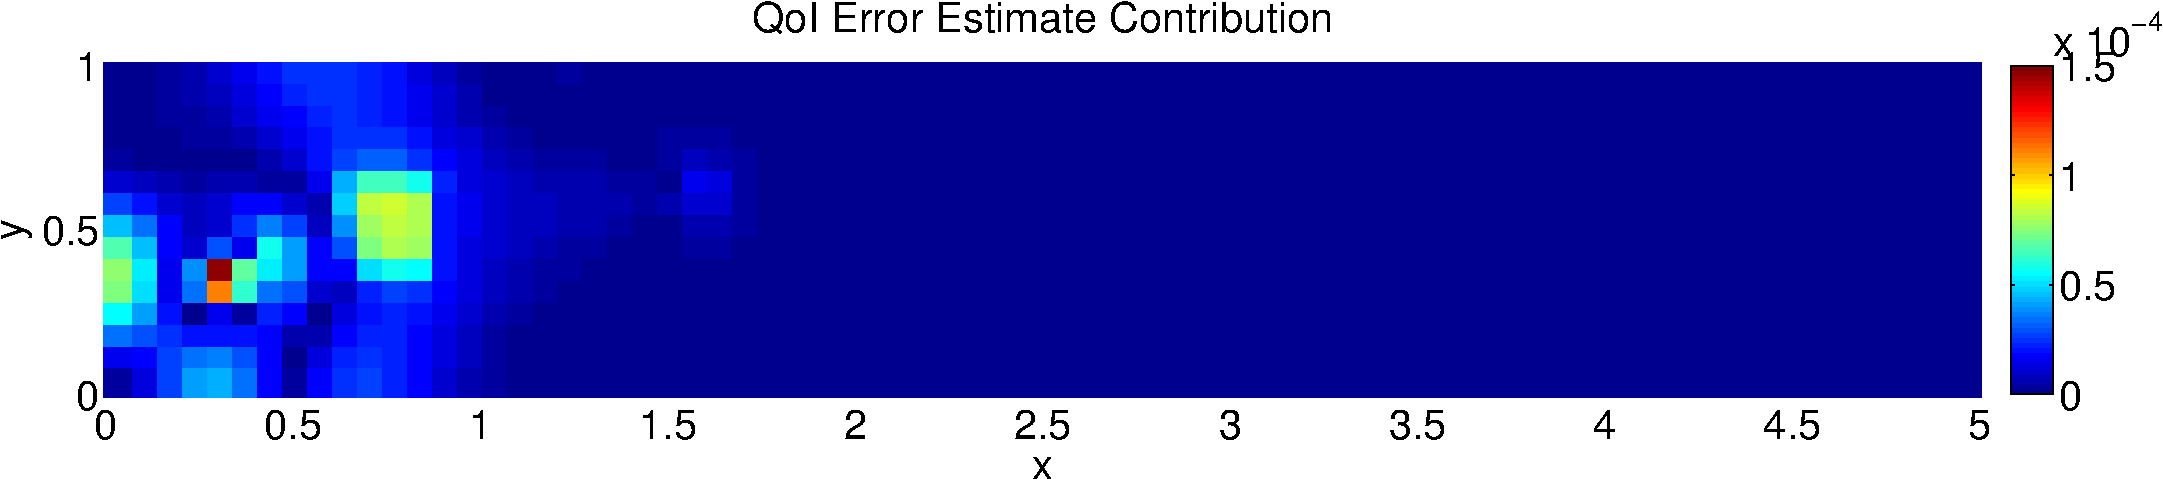
\includegraphics[width=0.8\textwidth]{vs_reg/err_breakdown_0p00001.pdf}}
\subfigure{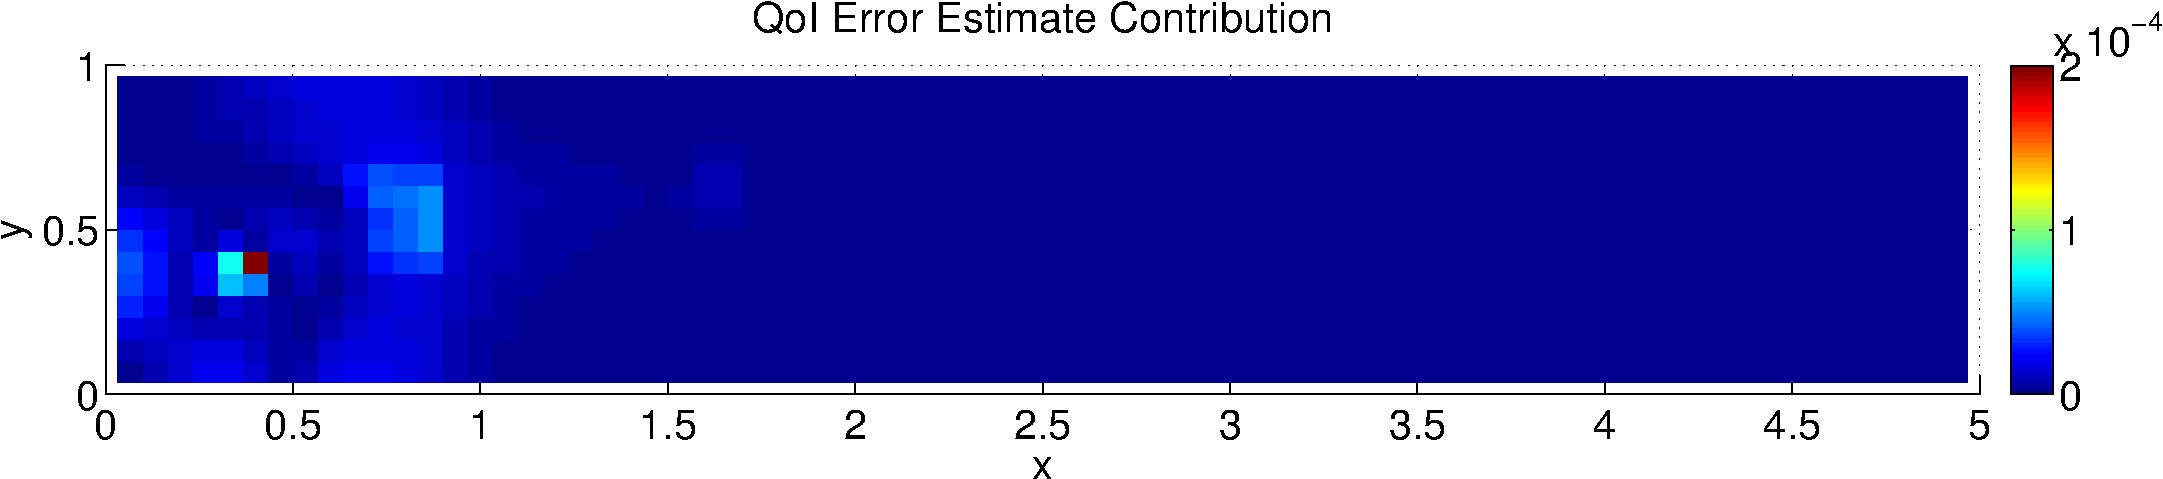
\includegraphics[width=0.8\textwidth]{vs_reg/err_breakdown_0p001.pdf}}
\subfigure{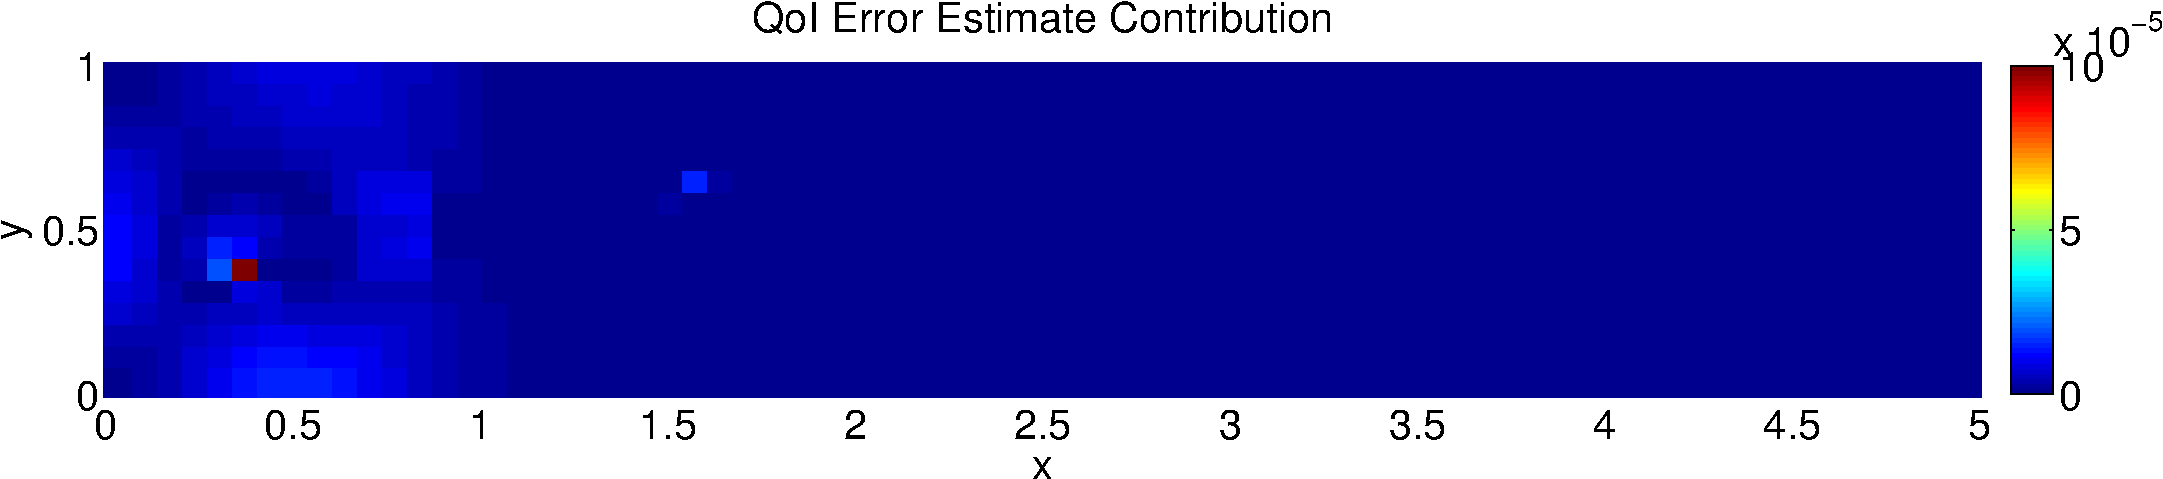
\includegraphics[width=0.8\textwidth]{vs_reg/err_breakdown_0p1.pdf}}
\caption{Element-wise decomposition of error estimates for varying $\beta$ \red{if keep make consistent}}
\label{fig:regStudy}
\end{figure}

%how to show, since a paper can't include animations or their flip-book equivalent? if showing how it picks out the important data points, how to justify only showing one (and not all from series of refinements), since linearization could contaminate error breakdown...
% -> vs measurements studies; vs qoi studies; vs reg study (?)
% -> DON'T HAVE: looking at contribution from regularization terms? indicator function QoI? boundary flux QoI? more physically meaningful boundary conditions? *different physics, one where effects propogate more*? 
	
%effectivity index (ratio of estimated to true error) plots/tables? (oden, prudhomme, et al mention such)

%...relate back to Chad's subspace of shared qoi-data importance (emphasis on shared importance...)? although his subspace was in parameter-space, not physical domain space...
%can we make an example where the qoi region is not pointed out for refinement? even with weak regularization

%try runs with inflow boundary conditions, which make more sense?
%gunzburger only has example with homo diri around the entire boundary...how to deal with BCs if boundary split between diri and neumann? -> poke 930...

%should these be re-run on finer meshes for prettier pictures?

%------------------------------------------------------------------------------%
\section{Scalar versus Field Parameters}  %\label{sec:xx}
%------------------------------------------------------------------------------%

The models considered need not differ in the physics included. In this section, we consider two models which differ in the space in the space to which the parameter belongs. The high-fidelity model 
\begin{equation}
k_d\nabla^2 u - \vec{V}\cdot\nabla u + k_ru^2= f(q),\quad q\in U,
\end{equation}
is again a single-species convection-diffusion-reaction equation with a nonlinear reaction term, where $k_d = 0.1$ is a diffusion coefficient and $k_r = -4.2$ is a reaction coefficient. The low-fidelity model
\begin{equation}
k_d\nabla^2 u - \vec{V}\cdot\nabla u + k_ru^2= f(q),\quad q\in\R
\end{equation}
differs from the high-fidelity model only in that the parameter is a scalar instead of a field.

%effect of linearization? the third point popping in and out in 4p2_deref is probably due to interplay of how fast third point's bump shrinks versus how fast the refinement percentage grows...
%can philisohically compare with chad's though, perhaps in param refinement, even though his is in parameter subspaces and ours is in physical space?
